\section*{Умова}

\begin{enumerate}
    \item Для зображення cameraman.tif застосувати логарифмічне перетворення
    $ f(x) = c \log(x + 1) $

    \begin{figure}[h]
        \begin{center}
            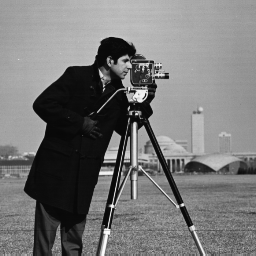
\includegraphics[width=0.4\textwidth]{cameraman.png}
            \caption*{Рис. 1 cameraman.tif}
        \end{center}
    \end{figure}

    \item Застосувати функцію препарування рис.2, визначивши точки перегину функції 
    препарування $x_{1}, x_{2}$, з метою підвищення контрастності перетвореного зображення.

    \begin{figure}[h]
        \begin{center}
            \begin{tikzpicture}
                \draw[thick,->] (0,0) -- (4.8,0) node[anchor=north west] {x axis};
                \draw[thick,->] (0,0) -- (0,4.8) node[anchor=south east] {y axis};
                \draw[red, ultra thick] (0,0) -- (1.6, 0) node[anchor=north] {$x_1$};
                \draw[red, ultra thick] (1.6, 0) -- (3.2, 3.2);
                \draw[black, dashed] (3.2, 3.2) -- (3.2, 0) node[anchor=north] {$x_2$};
                \draw[red, ultra thick] (3.2, 3.2) -- (4.7, 3.2);
            \end{tikzpicture}
            \caption*{Рис. 2 Функція препарування }
        \end{center}
    \end{figure}

\end{enumerate}

\pagebreak

\section*{Результати}

\begin{enumerate}
    \item Після застосування лагорифмічного перетворення з параметром $c = 1$ і застосування 
    лінійного контрастування отримуємо результат (див рис 3)
    \begin{figure}[h]
        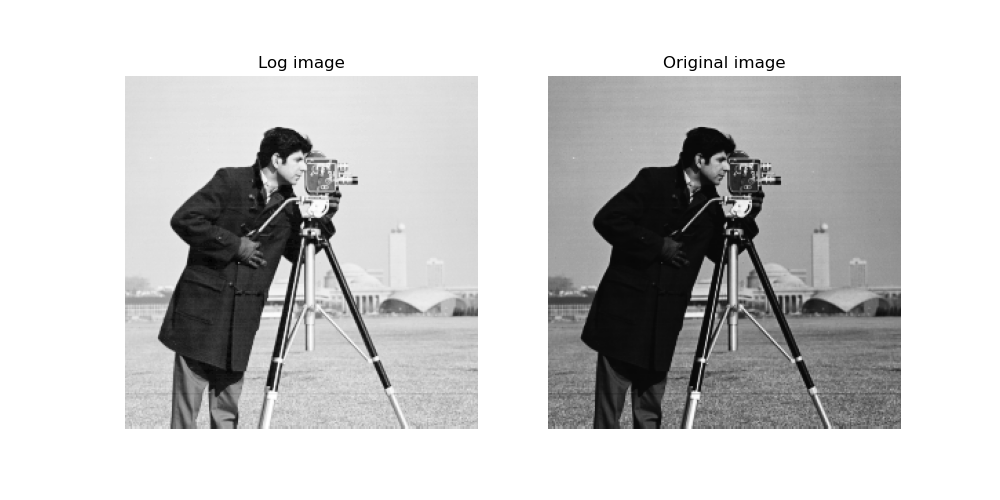
\includegraphics[width=\textwidth]{img_1.png}
        \caption*{Рис.3 Логарифмічне перетворення в порівнянні з оригіналом}
    \end{figure}

    \item Для визначення інтервалу препарування подивимось на гістограму зображення 
    (див рис 4)
    \begin{figure}[h]
        \begin{center}
            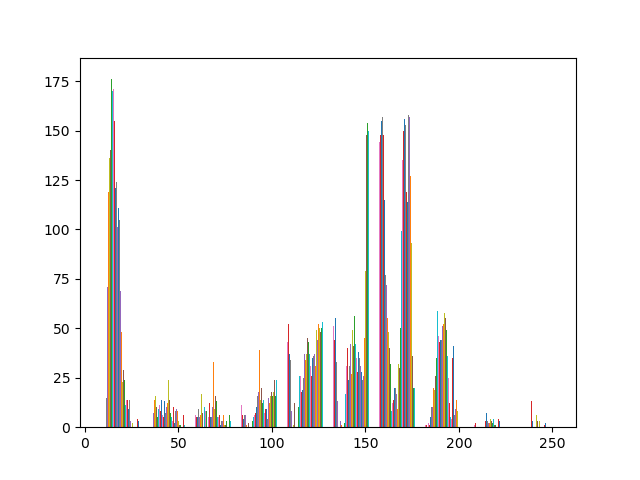
\includegraphics[width=0.5\textwidth]{hist.png}
        \end{center}
        \caption*{Рис.4 Гістограма зображення}
    \end{figure}
    
    
    Для препаруваня був обраний інтервал (5, 180). (див рис 5)
    \begin{figure}[h]
        \begin{center}
            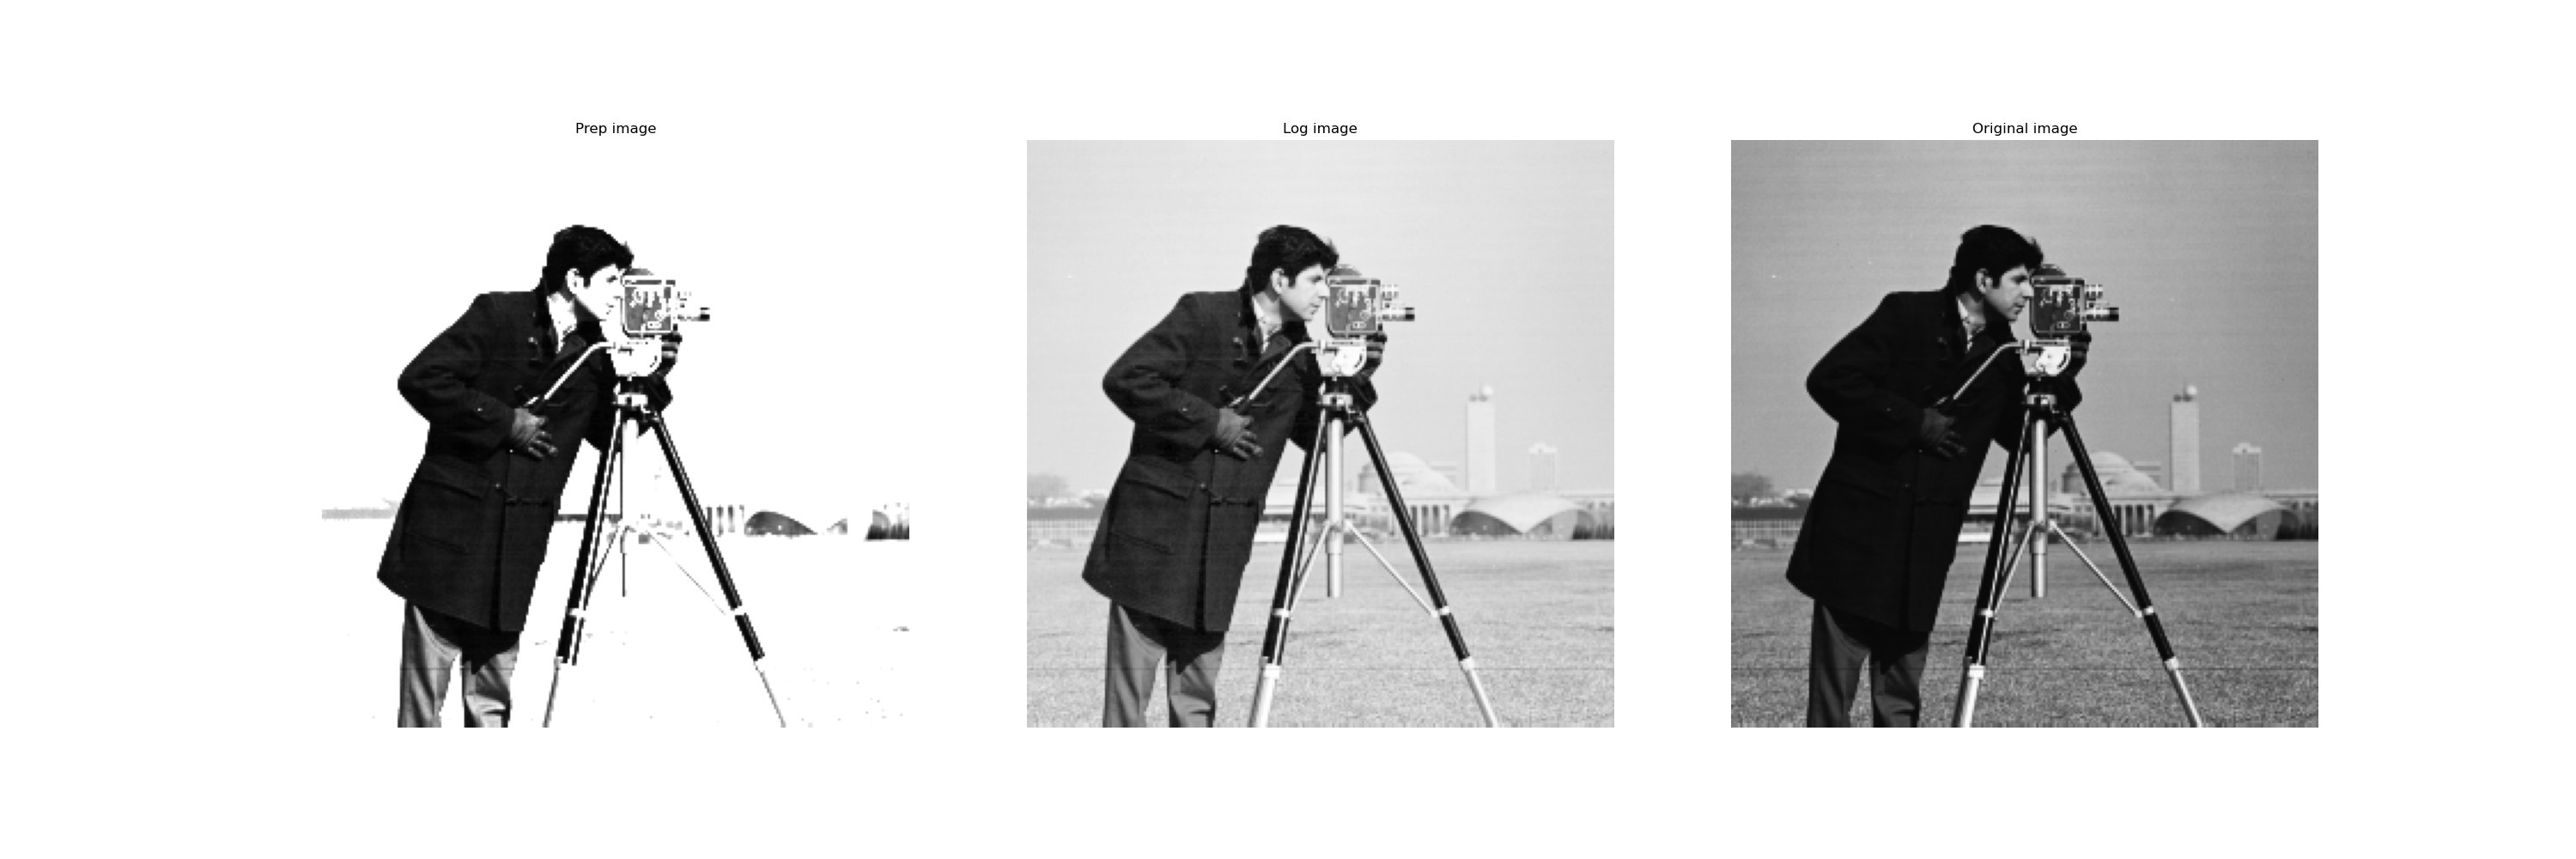
\includegraphics[width=\textwidth]{img_2.png}
        \end{center}
        \caption*{Рис.5 Зображення після препарування в порівнянні з минулими зображеннями}
    \end{figure}
\end{enumerate}
